
\section{Project Tango} \label{sec:theory_project_tango}

Project Tango ist eine Technologie Plattform für Android Tablets und Smartphones von Google’s Advanced Technology and Projects Group (ATAP). Das Ziel dieser Plattform ist es Motion Tracking (Positionierung), Depth Perception (Tiefeninformation/Pointcloud) und Area Learning (Lokalisierung) auf mobile Endgeräte zu bringen, um verschiedenste Anwendungs-Szenarien abzudecken. Typische Szenarien sind Indoor Navigation, Virtual Reality Anwendungen, Vermessungs- und Rekonstruktions Software und Augmented Reality Anwendungen.\\

Es ermöglicht in erster Linie ein Tracking von Positionsänderungen des Geräts im Raum und bietet somit eine genaue relative Lokalisierung. Mit Hilfe dieser Lokalisierung und der Hinzunahme von visuellen Merkmalen im Raum, ist das Gerät in der Lage, seine Umgebung kennenzulernen und gegebenenfalls die Lokalisierung zu korrigieren oder aber in einer bereits erlernten Umgebung zu ermitteln. Zusätzlich bietet Project Tango die Möglichkeit mit Hilfe eines Tiefensensors eine Pointcloud der Tiefeninformation pro Bildausschnitt zu liefern, um Anwendungen auch Räumliche Informationen bereitzustellen.  \citep{Proje19:online} \\

\subsection{Geräte und Hardware}

Da das Project Tango zum Zeitpunkt der Verfassung dieser Thesis noch unter Entwicklung steht, gibt es von Google die Entwickler Prototypen. Das Erste Gerät im Smartphone Format, welches in Abbildung \ref{fig:tango-device} rechts unten zu erkennen ist, wurde bereits durch eine neue Generation rechts oben ersetzt. Dieses 7\dq Tablet verfügt, wie in Abbildung \ref{fig:tango-device} links zu erkennen, über einen Infrarot Laser Projektor, eine Fisheye Camera und eine normale 4 Megapixel Kamera auf der Rückseite. Zudem sind, wie von aktuellen Smartphones bekannt, ein Beschleunigungssensor, Umgebungslichtsensor, Barometer, Kompass, GPS und ein Gyroskop verbaut. Das Gerät wird von einem NVIDIA Tegra K1 Prozessor betrieben und verfügt über 4GB Arbeitsspeicher. \citep{Proje19:online} Mit diesem Gerät wurden die später beschriebenen Techniken umgesetzt und evaluiert.  \\

\begin{figure}[h]
  \centering
	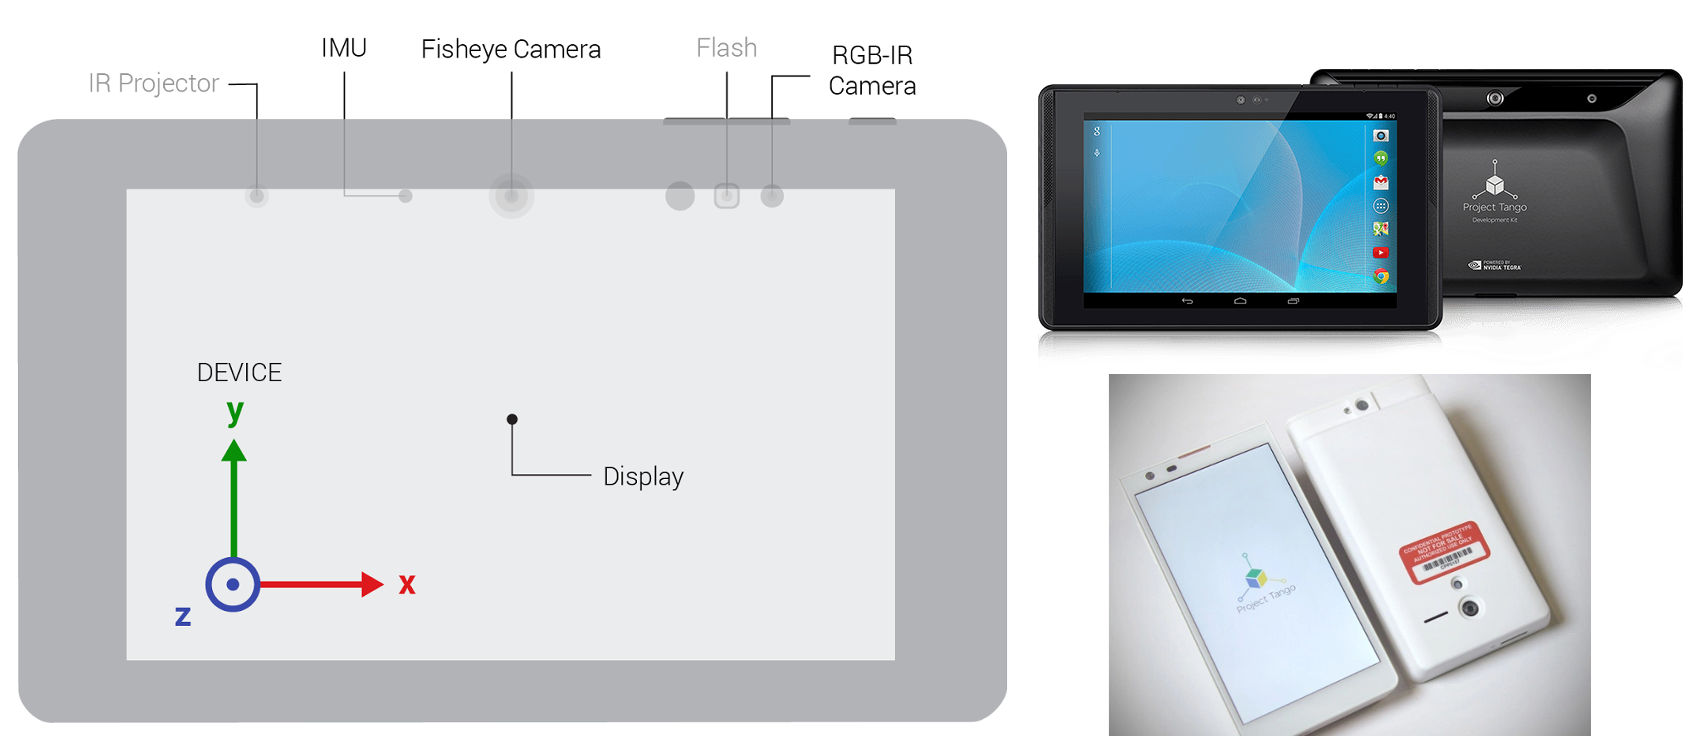
\includegraphics[width=1.0\textwidth]{content/images/theory/tango-device.png} 
  \caption{Links: schematischer Aufbau der Google Project Tango Hardware. Rechts: Das aktuelle Entwickler Gerät im Tablet Faktor (oben) und das alte Entwickler Gerät im Smartphone Faktor (unten). Übernommen von \citet{GoogleDevelopers:online}}
  \label{fig:tango-device}
\end{figure}

\subsection{Konzepte und Schnittstellen}

Generell betrachtet ist das Project Tango eine Plattform, die Computer Vision nutzt, um dem Gerät die Möglichkeit bietet seine relative Positionierung in der umgebenen Szene live zu bestimmen. Auf den Geräten kommt Googles Android zum Einsatz, weshalb zu beachten ist, dass es sich bei der Platform nur Bedingt um eine Echtzeit Umgebung handelt. Das liegt daran, dass der Linux Kernel keine Garantien für die zeitlich präzise Ausführung von Instruktionen  auf Grund von Scheduling geben kann. Google weist daher darauf hin, dass das System als \enquote{soft-realtime} betrachtet werden sollte. Daher sollten Messergebnisse verschiedener Sensoren unter Berücksichtigung ihrer Aufnahme Zeitstempel verwendet werden. \citep{GoogleDevelopersConcepts:online} \\

\subsubsection{Motion Tracking}

Um die relative Bewegung vom Start des Project Tango Systems bestimmen zu können nutzt es \enquote{visual-inertial odometry}. \citep{GoogleDevelopersConcepts:online}
Dabei handelt es sich um eine erweiterte Variante von Visual Odometry. 
Das von \citet{nister2004visual} veröffentlichte Verfahren Visual Odometry ist in der Lage aus einfachen Video Inhalten in Echtzeit die Bewegung der Kamera zu bestimmen. 
Hierzu werden zunächst übergreifende Features, zum Beispiel Punkte aus der \citet{harris1988combined} Kantenerkennung, über mehrere Bilder des Videos bestimmt, woraus mit Hilfe des 5-point Algorthmus und durch Answendung von RANSAC eine bestmögliche Approximation der Kamera Transformation bestimmt wird. \citep{nister2004visual} \\

Project Tango lässt an dieser Stelle die internen Sensoren zur Rotation, Orientierung und Bewegung mit in die Bestimmung der Kamera Transformation einfließen um so ein akurateres Ergebnis erziehlen zu können. Über eine längere Messzeit oder eine größere Entfernung vom Ursprung kann es jedoch zu kleinen Abweichungen kommen. Außerdem existiert zum aktullen Zeitpunkt noch ein \enquote{drift} Problem, was zu großen Messfehlern führen kann. Es wird jedoch versucht diese Probleme mit dem Konzept \enquote{Area Learning}, beschrieben in Kapitel \ref{subsec:area-learning}, zu lösen. \citep{GoogleDevelopersConcepts:online}
Wie genau das Verfahren aussieht, welche Techniken zur Feature Detection oder Feature Matching genutzt wird und welche Features hierfür erkannt werden ist nicht bekannt.  \\

\subsubsection{Deph Perception}

Zur Tiefenmessung ist die Project Tango Hardware mit einem kalibrierten Infrarot Laser Projektor ausgestattet. Dieser streut Infrarot Punkte mit einer Auflösung von 320 x 180 Punkten in den Raum, um dann, mit Hilfe von Aufnahmen der RGB Kamera, eine Punktewolke der Tiefeninformation zu bestimmen. Auf Grund einer ausgewogenen Konfiguration zwischen Messbereich, Messfehlern und dem Energieverbrauch, liegt der Messbereich der Sensorkombination, laut \citet{GoogleDevelopersConcepts:online}, zwischen einem halben und vier Metern. \\

Dadurch dass diese Technologie auf der Aufnahme von projiziertem Infrarot Licht basiert, ist ein Einsatz der Tiefenmessung außerhalb geschlossener Räume nicht möglich. \citep{GoogleDevelopersConcepts:online} Außerdem entstehen Messfehler durch reflektierende,  lichtabsorbierende oder zu komplex strukturierte Oberflächen, wie zum Beispiel Metalle, LCD Monitore oder Hochflor Teppiche. \\

Die zuvor erwähnten Punktewolken werden in dem eigens definierten XYZij Format von der Entwicklungsschnittstelle zurück gegeben. Dabei handelt es sich pro Punkt um die \(X\),\(Y\) und \(Z\) Koordinaten sowie der Spalte \(i \) und der Zeile \(j\). \citep{GoogleDevelopersConcepts:online} Man spricht dabei von einer organisierten Punktewolke, da durch die \(i\) und \(j\) Koordinaten die direkten Nachbarn, ausgehend von dem Aufnahmeblickwinkel, eines Punktes bestimmt werden können. Hieraus ist es möglich, die sogenannten \enquote{depth-maps} zu bestimmen, für die es viele verschiedene Computer Vision Verfahren zur Bestimmung von Objekten, Strukturen und Fluchtpunkten gibt !!! !!! . Die Ermittlung der Spalten \(i\) und Zeilen \(j\) sind jedoch laut \citet{GoogleDevelopersKnownIssues:online} noch nicht in den Schnittstellen enthalten.\\ 

\citet{GoogleDevelopersConcepts:online} weist darauf hin, dass das Generieren von Polygon basierten Rekonstruktionen noch nicht in den Schnittstellen enthalten sind. Es gibt jedoch freie Drittbibliotheken, wie das Robot Operating System \citep{ROS} oder die Point Cloud Library \citep{pcl}. Die für eine weitere Verarbeitung genutzt werden können.

\subsubsection{Area Learning} \label{subsec:area-learning}

Area Learning bezeichnet den Prozess indem Project Tango Geräte in der Lage sind durch visuelle Hinweise die umgebenen Welt kennenzulernen und auf die Position des Gerätes zu schließen. 
Es ermöglicht somit eine Unterstützung für Motion Tracking und löst das Problem das Gerät in einer bereits bekannten Umgebung zu lokalisieren, wie in Abbildung \ref{fig:area-learning} links zu erkennen.
Project Tango bietet außerdem die Möglichkeit diese visuellen Hinweise und Ihre Position im Raum in sogenannten \enquote{Area Description Files} zu speichern und wiederzuverwenden. \citep{GoogleDevelopersConcepts:online}\\

\begin{figure}[h]
  \centering
	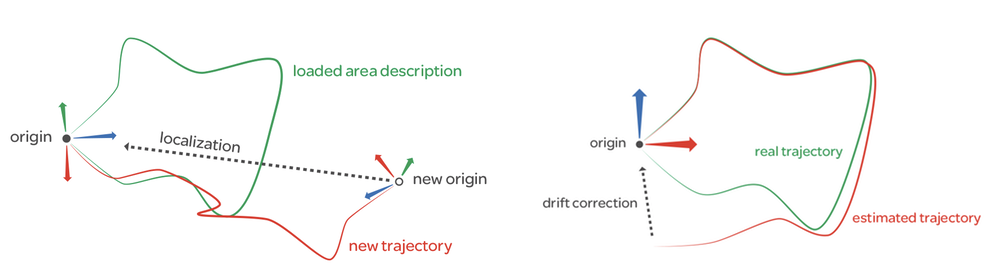
\includegraphics[width=1.0\textwidth]{content/images/theory/tango-area-learning.png} 
  \caption{Links: Lokalisierungsprozess durch Area Learning. Rechts: Korrigierung von Motion Tracking anhand gelernter Merkmale . Übernommen von \citet{GoogleDevelopers:online}}
  \label{fig:area-learning}
\end{figure}

Wie bereits erwähnt entstehen bei Motion Tracking Messfehler über eine längere Strecke. 
Während diese Strecke mit einem Project Tango Gerät abgelaufen wird, ermittelt es fortlaufend die Position und den Pfad, den der Nutzer im Raum gegangen ist. 
Erkennt es während der Strecke visuelle Merkmale vom Area Learning, wird der Pfad anhand der Positionen der Merkmale entsprechend angepasst. 
Project Tango unterscheidet hier zwischen zwei Manipulationen, \enquote{loop closures}, zur Zusammenführung des Pfads wenn ein Kreis gelaufen wurde, und \enquote{drift corrections}, um den erwähnten drift Effekt bei zu wenigen optischen Features im visual-inertial odometry. 
Die dirft correction ist in Abbildung \ref{fig:area-learning} rechts zu erkennen. \citep{GoogleDevelopersConcepts:online} \\

Auch bei diesem Prozess werden die genauen Details nicht näher erläutert und es nicht bekannt wie die area desciptions definiert sind oder was sie enthalten. \citep{GoogleDevelopersConcepts:online} weist jedoch darauf hin, dass auch wenn die Area Desciptions Files keine direkten Bilder enthalten, es möglich sei, Rückschlüsse auf die gelernte Umgebung ziehen zu können. \\

\subsection{Einordnung zu Augmented Reality}

Da sowohl die Grundlagen aus dem Bereich Augmented Reality und die technische Basis von Project Tango bekannt ist, kann die Project Tango Hardware bezüglich Augmented Reality näher eingeordnet werden. Bei der Hardware handelt es sich um ein hand-held Gerät, welches mit einer see-through Display Technologie Augmented Reality Anwendungen ermöglicht. Hierfür kann wahlweise die normale RGB Kamera oder die Graustufen Fish-Eye Kamera verwendet werden. Als Tracking Technologie wird hier eine hybride optische Variante angewendet, die Visual Odometry mit der Fish-Eye Kamera durch interne Sensoren für die Rotation, Orientierung und Bewegung kombiniert. Außerdem wird gegebenenfalls dieses Verfahren durch Googles Area Learning Mechanismus angereichert um Messfehler entgegenzuwirken. Die Eingabe erfolgt dabei durch den Touchscreen des Tablets. Eine Interaktion mit Hilfe von optischer Gestenerkennung oder anhand der Tiefeninformationen zudem auch möglich. \\
